\chapter{Экспериментальная валидация}\label{ch:experiment}

% TODO (M6): ~5 страниц — ЦЕНТРАЛЬНАЯ практическая глава.
% Структура:
%   7.1 Аппаратный стенд
%       — компоненты: ESP32 DevKit V1 (WROOM-32), Waveshare 2.13" V4 (SSD1680),
%         INA219 (CJMCU, 0.1 Ω шунт);
%       — схема подключения (3 группы соединений: SPI к HAT, I²C к INA219,
%         силовая через шунт);
%       — фото стенда (общий вид + крупно INA219).
%   7.2 Прошивка ESP32 (расширение)
%       — опкоды 0x01-0x0E (см. §A.1 Приложения);
%       — измерительный pipeline через 0x0E BENCH_RUN;
%       — особенность: 0x22=0xC7 для нашего custom LUT (не перезаписывается).
%   7.3 Фотостанд для измерения ghost
%       — кожух, освещение, камера/iPhone, фиксированное расстояние;
%       — pipeline ImageJ / scikit-image для извлечения SSIM/residual.
%   7.4 Протокол измерения
%       — 5 baseline (B0..B4: Waveshare full, Waveshare fast, custom static,
%         content-adaptive, temp+content-adaptive);
%       — 10 сценариев × 50 повторов = 2500 измерений по baseline;
%       — таблица: среднее E, медиана G, max τ, std.
%   7.5 Сравнение симулированного и реального Парето
%       — наложение sim Парето из §6 и измеренного на стенде;
%       — анализ расхождений: систематические смещения, выбросы;
%       — обсуждение пределов применимости surrogate-модели.

\section*{Заглушка}

Раздел будет наполнен на этапе~M6 в соответствии с Chapter Plan
(см. \texttt{.ai-factory/RESEARCH.md}).

\begin{figure}[ht]
    \centering
    % TikZ-схема фотостанда для гл. 7 § 7.3.
% Подключается через % TikZ-схема фотостанда для гл. 7 § 7.3.
% Подключается через % TikZ-схема фотостанда для гл. 7 § 7.3.
% Подключается через \input{figures/diagrams/photo_stand.tex}.
\begin{tikzpicture}[
    every node/.style={font=\footnotesize},
    box/.style={draw, thick, fill=gray!8},
    phone/.style={draw, thick, fill=white, rounded corners=1.5pt,
                  minimum width=40mm, minimum height=10mm},
    epd/.style={draw, thick, fill=white, minimum width=34mm, minimum height=8mm},
    label/.style={font=\scriptsize, align=left, inner sep=1pt},
    sidelight/.style={draw=orange!80!black, thick, fill=yellow!50,
                      minimum width=4mm, minimum height=8mm},
]

% --- Корпус коробки (вид сбоку, разрез) -----------------------------
% Стенки и дно — верх открыт.
\draw[box]
    (-4.0, -2.8) -- (-4.0, 1.6)        % левая стенка
    (-4.0, -2.8) -- (4.0, -2.8)        % дно
    (4.0, -2.8) -- (4.0, 1.6);         % правая стенка

% Чёрное матовое дно (штриховка внутри)
\fill[pattern=north east lines, pattern color=black!70]
    (-3.85, -2.7) rectangle (3.85, -2.4);

% Жирные внутренние стенки = «чёрные стенки»
\draw[line width=1.8pt, black] (-3.85, -2.7) -- (-3.85, 1.45);
\draw[line width=1.8pt, black] ( 3.85, -2.7) -- ( 3.85, 1.45);

% --- Телефон лежит СВЕРХУ коробки, перекрывая отверстие -------------
% (объектив снизу телефона смотрит в открытое отверстие коробки)
\node[phone] (phone) at (0, 2.0) {};
\node[font=\scriptsize] at (0, 2.0) {Телефон (камерой вниз)};

% Объектив (снизу телефона, внутрь коробки)
\filldraw[fill=black!50] (0, 1.55) circle (1.8mm);
\node[label] at (0.55, 1.55) [right] {объектив};

% Отверстие в верхе коробки — рисуем разрыв стенок (уже сделано выше)
\node[label, align=center] at (-3.0, 2.4) {верх открыт\\(отверстие)};
\draw[->, thin, gray] (-2.55, 2.30) -- (-1.0, 1.65);

% --- Боковое освещение (телефон-фонарик с диффузором или лампа) -----
\node[sidelight, rotate=-30] (lampL) at (-3.0, 0.4) {};
\node[sidelight, rotate=30]  (lampR) at ( 3.0, 0.4) {};
\node[label, align=center] at (-3.0, 1.05) {боковой\\свет};
\node[label, align=center] at ( 3.0, 1.05) {боковой\\свет};

% Лучи света от боковых источников на EPD (диффузные пунктиры)
\draw[-{Stealth[length=1.5mm]}, dashed, orange!70!black, thick]
    (-2.7, 0.2) -- (-0.7, -2.05);
\draw[-{Stealth[length=1.5mm]}, dashed, orange!70!black, thick]
    ( 2.7, 0.2) -- ( 0.7, -2.05);

% --- EPD-панель в центре дна, лицом вверх ---------------------------
\node[epd] (epd) at (-0.6, -2.18) {EPD (Waveshare 2.13"V4)};

% --- Калибровочный квадрат рядом с EPD ------------------------------
\filldraw[draw=black, very thick, fill=white] (2.0, -2.35) rectangle (2.5, -1.85);
\draw[->, thin, gray] (2.65, -1.65) -- (2.40, -1.95);
\node[label, align=left] at (2.7, -1.45) [right] {калибр.\\квадрат\\(опц.)};

% --- Расстояние от объектива до EPD (двойная стрелка слева) ---------
\draw[<->, thick, red!80!black] (-3.4, 1.55) -- (-3.4, -2.18)
    node[midway, left, label, text=red!80!black] {15--20\,см};

% --- Подпись чёрного дна -------------------------------------------
\draw[->, thin, gray] (-3.2, -3.05) -- (-3.4, -2.55);
\node[label, align=left] at (-3.2, -3.18) {чёрное матовое дно};

% --- Заголовок вида ------------------------------------------------
\node[label] at (0, -3.55) [font=\scriptsize\itshape] {вид сбоку (разрез коробки)};

\end{tikzpicture}
.
\begin{tikzpicture}[
    every node/.style={font=\footnotesize},
    box/.style={draw, thick, fill=gray!8},
    phone/.style={draw, thick, fill=white, rounded corners=1.5pt,
                  minimum width=40mm, minimum height=10mm},
    epd/.style={draw, thick, fill=white, minimum width=34mm, minimum height=8mm},
    label/.style={font=\scriptsize, align=left, inner sep=1pt},
    sidelight/.style={draw=orange!80!black, thick, fill=yellow!50,
                      minimum width=4mm, minimum height=8mm},
]

% --- Корпус коробки (вид сбоку, разрез) -----------------------------
% Стенки и дно — верх открыт.
\draw[box]
    (-4.0, -2.8) -- (-4.0, 1.6)        % левая стенка
    (-4.0, -2.8) -- (4.0, -2.8)        % дно
    (4.0, -2.8) -- (4.0, 1.6);         % правая стенка

% Чёрное матовое дно (штриховка внутри)
\fill[pattern=north east lines, pattern color=black!70]
    (-3.85, -2.7) rectangle (3.85, -2.4);

% Жирные внутренние стенки = «чёрные стенки»
\draw[line width=1.8pt, black] (-3.85, -2.7) -- (-3.85, 1.45);
\draw[line width=1.8pt, black] ( 3.85, -2.7) -- ( 3.85, 1.45);

% --- Телефон лежит СВЕРХУ коробки, перекрывая отверстие -------------
% (объектив снизу телефона смотрит в открытое отверстие коробки)
\node[phone] (phone) at (0, 2.0) {};
\node[font=\scriptsize] at (0, 2.0) {Телефон (камерой вниз)};

% Объектив (снизу телефона, внутрь коробки)
\filldraw[fill=black!50] (0, 1.55) circle (1.8mm);
\node[label] at (0.55, 1.55) [right] {объектив};

% Отверстие в верхе коробки — рисуем разрыв стенок (уже сделано выше)
\node[label, align=center] at (-3.0, 2.4) {верх открыт\\(отверстие)};
\draw[->, thin, gray] (-2.55, 2.30) -- (-1.0, 1.65);

% --- Боковое освещение (телефон-фонарик с диффузором или лампа) -----
\node[sidelight, rotate=-30] (lampL) at (-3.0, 0.4) {};
\node[sidelight, rotate=30]  (lampR) at ( 3.0, 0.4) {};
\node[label, align=center] at (-3.0, 1.05) {боковой\\свет};
\node[label, align=center] at ( 3.0, 1.05) {боковой\\свет};

% Лучи света от боковых источников на EPD (диффузные пунктиры)
\draw[-{Stealth[length=1.5mm]}, dashed, orange!70!black, thick]
    (-2.7, 0.2) -- (-0.7, -2.05);
\draw[-{Stealth[length=1.5mm]}, dashed, orange!70!black, thick]
    ( 2.7, 0.2) -- ( 0.7, -2.05);

% --- EPD-панель в центре дна, лицом вверх ---------------------------
\node[epd] (epd) at (-0.6, -2.18) {EPD (Waveshare 2.13"V4)};

% --- Калибровочный квадрат рядом с EPD ------------------------------
\filldraw[draw=black, very thick, fill=white] (2.0, -2.35) rectangle (2.5, -1.85);
\draw[->, thin, gray] (2.65, -1.65) -- (2.40, -1.95);
\node[label, align=left] at (2.7, -1.45) [right] {калибр.\\квадрат\\(опц.)};

% --- Расстояние от объектива до EPD (двойная стрелка слева) ---------
\draw[<->, thick, red!80!black] (-3.4, 1.55) -- (-3.4, -2.18)
    node[midway, left, label, text=red!80!black] {15--20\,см};

% --- Подпись чёрного дна -------------------------------------------
\draw[->, thin, gray] (-3.2, -3.05) -- (-3.4, -2.55);
\node[label, align=left] at (-3.2, -3.18) {чёрное матовое дно};

% --- Заголовок вида ------------------------------------------------
\node[label] at (0, -3.55) [font=\scriptsize\itshape] {вид сбоку (разрез коробки)};

\end{tikzpicture}
.
\begin{tikzpicture}[
    every node/.style={font=\footnotesize},
    box/.style={draw, thick, fill=gray!8},
    phone/.style={draw, thick, fill=white, rounded corners=1.5pt,
                  minimum width=40mm, minimum height=10mm},
    epd/.style={draw, thick, fill=white, minimum width=34mm, minimum height=8mm},
    label/.style={font=\scriptsize, align=left, inner sep=1pt},
    sidelight/.style={draw=orange!80!black, thick, fill=yellow!50,
                      minimum width=4mm, minimum height=8mm},
]

% --- Корпус коробки (вид сбоку, разрез) -----------------------------
% Стенки и дно — верх открыт.
\draw[box]
    (-4.0, -2.8) -- (-4.0, 1.6)        % левая стенка
    (-4.0, -2.8) -- (4.0, -2.8)        % дно
    (4.0, -2.8) -- (4.0, 1.6);         % правая стенка

% Чёрное матовое дно (штриховка внутри)
\fill[pattern=north east lines, pattern color=black!70]
    (-3.85, -2.7) rectangle (3.85, -2.4);

% Жирные внутренние стенки = «чёрные стенки»
\draw[line width=1.8pt, black] (-3.85, -2.7) -- (-3.85, 1.45);
\draw[line width=1.8pt, black] ( 3.85, -2.7) -- ( 3.85, 1.45);

% --- Телефон лежит СВЕРХУ коробки, перекрывая отверстие -------------
% (объектив снизу телефона смотрит в открытое отверстие коробки)
\node[phone] (phone) at (0, 2.0) {};
\node[font=\scriptsize] at (0, 2.0) {Телефон (камерой вниз)};

% Объектив (снизу телефона, внутрь коробки)
\filldraw[fill=black!50] (0, 1.55) circle (1.8mm);
\node[label] at (0.55, 1.55) [right] {объектив};

% Отверстие в верхе коробки — рисуем разрыв стенок (уже сделано выше)
\node[label, align=center] at (-3.0, 2.4) {верх открыт\\(отверстие)};
\draw[->, thin, gray] (-2.55, 2.30) -- (-1.0, 1.65);

% --- Боковое освещение (телефон-фонарик с диффузором или лампа) -----
\node[sidelight, rotate=-30] (lampL) at (-3.0, 0.4) {};
\node[sidelight, rotate=30]  (lampR) at ( 3.0, 0.4) {};
\node[label, align=center] at (-3.0, 1.05) {боковой\\свет};
\node[label, align=center] at ( 3.0, 1.05) {боковой\\свет};

% Лучи света от боковых источников на EPD (диффузные пунктиры)
\draw[-{Stealth[length=1.5mm]}, dashed, orange!70!black, thick]
    (-2.7, 0.2) -- (-0.7, -2.05);
\draw[-{Stealth[length=1.5mm]}, dashed, orange!70!black, thick]
    ( 2.7, 0.2) -- ( 0.7, -2.05);

% --- EPD-панель в центре дна, лицом вверх ---------------------------
\node[epd] (epd) at (-0.6, -2.18) {EPD (Waveshare 2.13"V4)};

% --- Калибровочный квадрат рядом с EPD ------------------------------
\filldraw[draw=black, very thick, fill=white] (2.0, -2.35) rectangle (2.5, -1.85);
\draw[->, thin, gray] (2.65, -1.65) -- (2.40, -1.95);
\node[label, align=left] at (2.7, -1.45) [right] {калибр.\\квадрат\\(опц.)};

% --- Расстояние от объектива до EPD (двойная стрелка слева) ---------
\draw[<->, thick, red!80!black] (-3.4, 1.55) -- (-3.4, -2.18)
    node[midway, left, label, text=red!80!black] {15--20\,см};

% --- Подпись чёрного дна -------------------------------------------
\draw[->, thin, gray] (-3.2, -3.05) -- (-3.4, -2.55);
\node[label, align=left] at (-3.2, -3.18) {чёрное матовое дно};

% --- Заголовок вида ------------------------------------------------
\node[label] at (0, -3.55) [font=\scriptsize\itshape] {вид сбоку (разрез коробки)};

\end{tikzpicture}

    \caption{Схема фотостанда для измерения reflectance EPD-панели:
        картонный корпус с чёрными матовыми стенками и дном устраняет
        паразитные отражения; телефон лежит сверху коробки камерой вниз
        через отверстие в верхе; боковые источники света дают мягкое
        освещение под углом, минимизирующее блики на глянцевой
        поверхности EPD; панель размещается лицом вверх в центре дна на
        расстоянии 15--20\,см от объектива; необязательный калибровочный
        квадрат рядом с EPD служит для нормировки яркости снимков}
    \label{fig:photo-stand}
\end{figure}

\begin{figure}[ht]
    \centering
    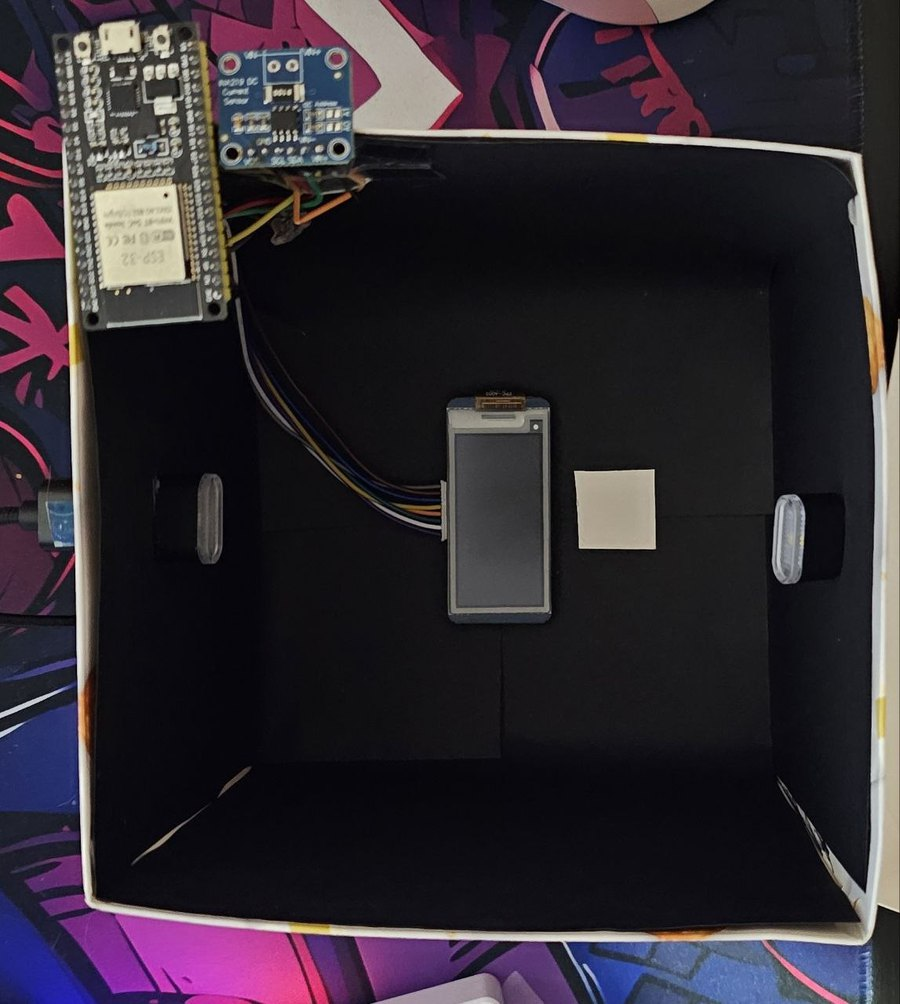
\includegraphics[width=0.5\textwidth]{figures/raw_photos/stand_overview.jpg}
    \caption{Общий вид собранного стенда (съёмка сверху): плата
        ESP32~DevKit и датчик тока INA219 закреплены на краю картонного
        корпуса; шлейф соединяет ESP32 с панелью Waveshare~2.13"~V4,
        лежащей лицом вверх по центру; справа~--- белый калибровочный
        квадрат; по бокам~--- USB-светодиодные источники диффузной подсветки}
    \label{fig:stand-photo}
\end{figure}

\begin{figure}[ht]
    \centering
    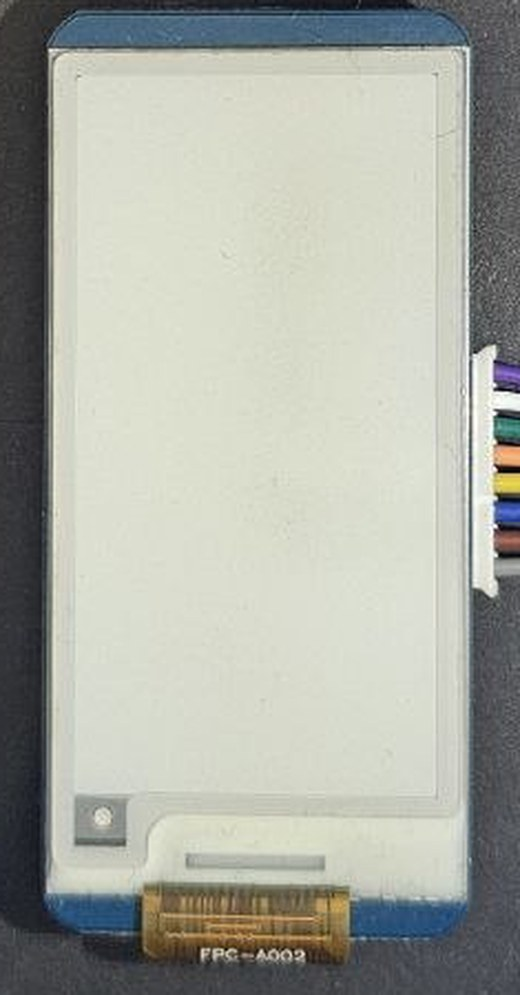
\includegraphics[height=42mm]{figures/raw_photos/epd_white.jpg}
    \hspace{8mm}
    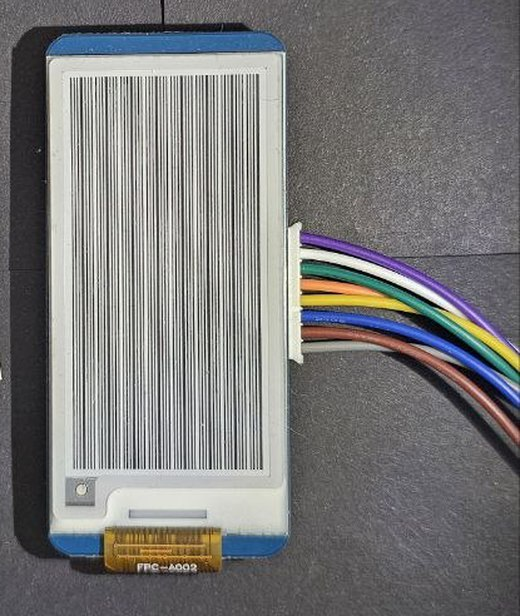
\includegraphics[height=42mm]{figures/raw_photos/epd_checker.jpg}
    \caption{Снимки панели на стенде (слева~--- чистое белое поле WW после
        полного заводского обновления, низкий контраст e-ink
        $\rho_{\max} \approx 0{,}40$; справа~--- отрисованный тестовый
        паттерн, демонстрация корректной пиксельной адресации). Рядом с
        панелью виден белый калибровочный квадрат для яркостной нормировки}
    \label{fig:epd-captures}
\end{figure}

\begin{figure}[ht]
    \centering
    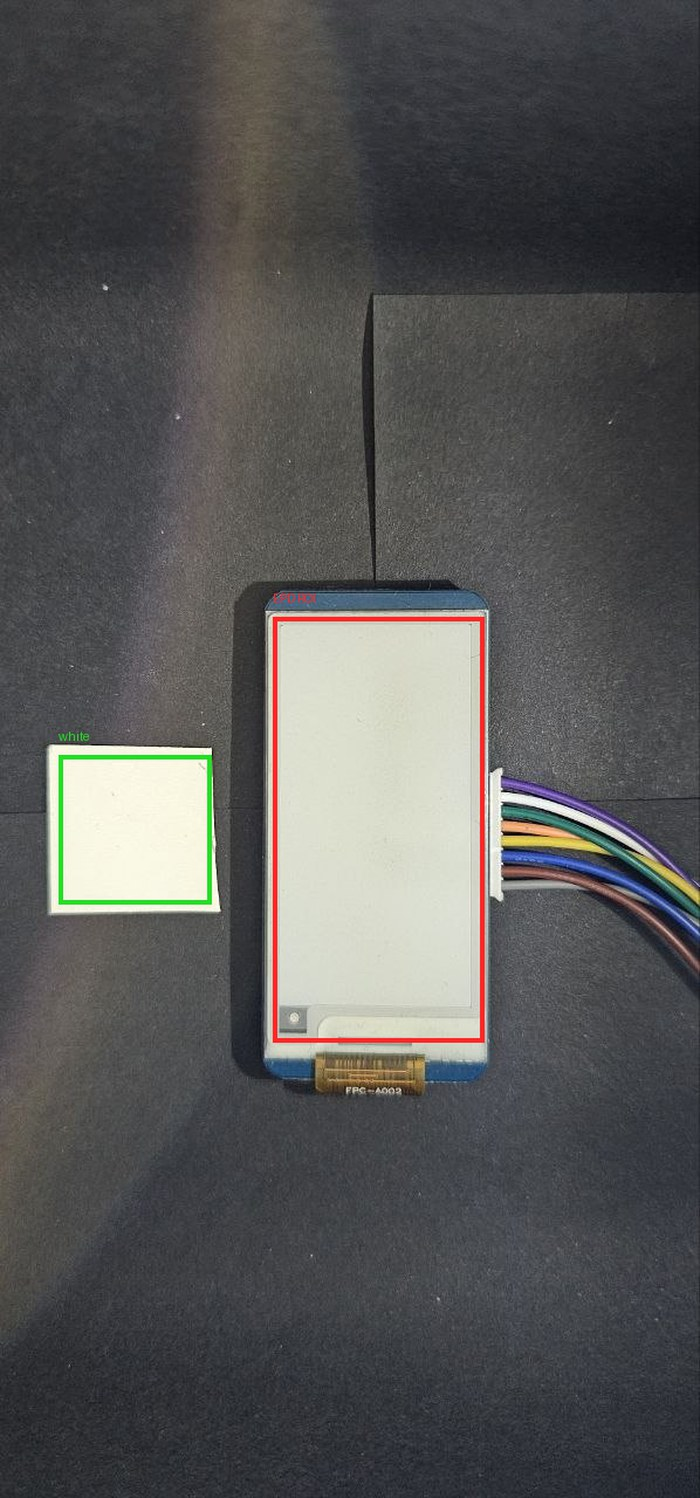
\includegraphics[width=0.5\textwidth]{figures/raw_photos/roi_overlay.jpg}
    \caption{Калибровка области интереса (ROI) по эталонному снимку белого
        поля: красной рамкой выделена активная область дисплея
        ($122 \times 250$ после выпрямления), зелёной~--- белый
        калибровочный квадрат. Координаты определяются автоматически
        (скрипт \texttt{scripts/calibrate\_roi.py}) и фиксируются для всей
        измерительной кампании, поскольку камера и панель неподвижны}
    \label{fig:roi-overlay}
\end{figure}
